\chapter{सूक्ष्मजैविक उपापचय और जैवफ़िल्में}\label{ch:b2:microbial-metabolism}

काँच के किसी बेलन में तालाब की कीचड़, थोड़ा कतरा हुआ काग़ज़, एक अंडे की
ज़र्दी और पानी भरिए और उसे खिड़की पर रख दीजिए। कुछ ही सप्ताहों में वह
रंगीन पट्टियों में बँट जाता है: ऊपर हरी शैवाल, एक ज़ंग-रंगी परत, एक
बैंगनी पट्टी, उससे नीचे एक हरी, और तल पर काली सल्फाइड कीचड़। प्रकाश के
सिवा कुछ भी नहीं डाला गया। हर पट्टी एक आबादी है जो किसी अलग रसायन पर
जीती है --- ऑक्सीजन पर, नाइट्रेट पर, सल्फेट पर, सल्फाइड पर, हाइड्रोजन
पर --- और हर एक अगली को पालती है। वह बेलन लघु रूप में सूक्ष्मजैविक जगत्
है: ऐसी कोशिकाएँ जो लगभग किसी भी ऐसे पदार्थ-युग्म से अपनी ऊर्जा कमा
लेती हैं जो इलेक्ट्रॉनों का विनिमय कर सके, और जो मिलकर ग्रह के रासायनिक
चक्र चलाती हैं। यह अध्याय उस ऊर्जाविज्ञान का तर्क, सूक्ष्मजैविक वृद्धि
की बलगतिकी, और सतहों पर सूक्ष्मजीवों का सामूहिक जीवन प्रस्तुत करता है
--- और उनमें से अधिकांश वास्तव में इसी तरह जीते हैं।

\section{जीविका कमाने के ढंग}

\begin{definition}[पोषी प्रकार]\label{def:b2:microbial-metabolism:trophic}
\index{रसपोषी}\index{प्रकाशपोषी}\index{शिलापोषी}\index{कार्बनिकपोषी}
किसी जीव का वर्गीकरण तीन उत्तरों से होता है। उसका \emph{ऊर्जा स्रोत}:
प्रकाश (\emph{प्रकाशपोषी}) या रासायनिक अभिक्रियाएँ (\emph{रसपोषी})।
उसका \emph{इलेक्ट्रॉन स्रोत}: अकार्बनिक पदार्थ --- $\mathrm{H_2}$,
$\mathrm{H_2S}$, $\mathrm{NH_4^+}$, $\mathrm{Fe^{2+}}$, जल ---
(\emph{शिलापोषी}) या कार्बनिक अणु (\emph{कार्बनिकपोषी})। उसका
\emph{कार्बन स्रोत}: $\mathrm{CO_2}$ (\emph{स्वपोषी}) या कार्बनिक
कार्बन (\emph{परपोषी})। पौधे और सायनोजीवाणु
प्रकाशशिलास्वपोषी हैं; प्राणी, कवक और \emph{E.~coli}
रसकार्बनिकपरपोषी हैं; नाइट्रीकारी और गंधक-ऑक्सीकारी
जीवाणु रसशिलास्वपोषी हैं, जो अँधेरे में खनिजों के ऑक्सीकरण से पाई ऊर्जा
से $\mathrm{CO_2}$ से अपना कार्बनिक पदार्थ बनाते हैं। लगभग हर संयोजन
प्राक्केंद्रकियों में कहीं न कहीं मिलता है; सुकेंद्रकी केवल दो घेरते हैं।
\end{definition}

\begin{theorem}[किसी अपचयोपचय युग्म की ऊर्जा]\label{thm:b2:microbial-metabolism:redox}
\index{अपचयोपचय विभव}\index{इलेक्ट्रॉन मीनार}
हर ऊर्जादायी उपापचय इलेक्ट्रॉनों को किसी \emph{दाता} युग्म से किसी
\emph{ग्राही} युग्म तक ले जाता है। हर युग्म का एक मानक विभव
$E^{\circ\prime}$ है (pH 7 पर): वह जितना अधिक ऋणात्मक, उतनी ही सहजता से
वह इलेक्ट्रॉन देता है। इलेक्ट्रॉनों के $n$ मोल $E_d$ पर किसी दाता से
$E_a$ पर किसी ग्राही तक हस्तांतरित करने पर इतनी मानक मुक्त ऊर्जा
निकलती है:
\[
\Delta G^{\circ\prime} = -\,n F\,(E_a - E_d), \qquad F = \qty{96.5}{kJ/V/mol},
\]
यानी उपज \emph{\omterm{thm:b2:microbial-metabolism:redox}{इलेक्ट्रॉन मीनार}} पर दोनों युग्मों के बीच की
ऊर्ध्वाधर दूरी के समानुपाती है। \qty{+0.82}{V} पर
$\mathrm{O_2/H_2O}$ और \qty{-0.43}{V} पर $\mathrm{CO_2}$/ग्लूकोज़
लेने पर, ग्लूकोज़ के एक अणु के 24 इलेक्ट्रॉन
$24\times 96.5\times 1.25 = \qty{2900}{kJ/mol}$ देते हैं; वही
इलेक्ट्रॉन सल्फेट ($\mathrm{SO_4^{2-}/H_2S}$, \qty{-0.22}{V}) को सौंपे
जाएँ तो केवल $24\times 96.5\times 0.21 = \qty{490}{kJ/mol}$ देते हैं।
\end{theorem}
\begin{proof}
अभिक्रिया दाता$_{\text{अपचयित}}$ + ग्राही$_{\text{ऑक्सीकृत}}$
$\to$ दाता$_{\text{ऑक्सीकृत}}$ + ग्राही$_{\text{अपचयित}}$ के लिए,
मुक्त-ऊर्जा परिवर्तन वह कार्य है जो इलेक्ट्रॉन आवेश के $n$ मोल, यानी $nF$,
विभवांतर $E_a - E_d$ से गिरकर करते हैं, और चिह्न-परिपाटी यह है कि किसी
स्वतःप्रवर्तित हस्तांतरण (इलेक्ट्रॉन अधिक धनात्मक युग्म की ओर) में
$\Delta G < 0$ होता है। यह वर्ष 1 के खंड का नर्न्स्ट संबंध है, जो दो
अर्ध-अभिक्रियाओं पर लगाया गया है।
\end{proof}

\begin{omfigure}
\begin{tikzpicture}[every node/.style={font=\scriptsize}, y=6cm]
  \draw[thick, ->] (0,-0.55) -- (0,0.95) node[above] {$E^{\circ\prime}$ (V)};
  \foreach \v in {-0.4,-0.2,0,0.2,0.4,0.6,0.8} \draw (-0.08,\v) -- (0.08,\v) node[right, xshift=0.05cm] {\v};
  % donors on the right: value/label position/text
  \foreach \v/\y/\l in {-0.43/-0.49/{$\mathrm{CO_2}$/glucose}, -0.42/-0.40/{$2\mathrm{H^+/H_2}$}, -0.32/-0.31/{$\mathrm{NAD^+/NADH}$}, -0.27/-0.22/{$\mathrm{S^0/H_2S}$}, 0.03/0.03/{fumarate/succinate}, 0.34/0.34/{$\mathrm{NO_2^-/NH_4^+}$}}
    { \draw[omDef, thick] (0.8,\v) -- (1.6,\v); \draw[omDef] (1.6,\v) -- (1.85,\y); \node[omDef, anchor=west] at (1.9,\y) {\l}; }
  % acceptors on the left
  \foreach \v/\y/\l in {-0.24/-0.29/{$\mathrm{CO_2/CH_4}$}, -0.22/-0.17/{$\mathrm{SO_4^{2-}/H_2S}$}, 0.43/0.43/{$\mathrm{NO_3^-/NO_2^-}$}, 0.74/0.69/{$\mathrm{NO_3^-/N_2}$}, 0.77/0.77/{$\mathrm{Fe^{3+}/Fe^{2+}}$}, 0.82/0.86/{$\mathrm{O_2/H_2O}$}}
    { \draw[omThm, thick] (-1.6,\v) -- (-0.8,\v); \draw[omThm] (-1.6,\v) -- (-1.85,\y); \node[omThm, anchor=east] at (-1.9,\y) {\l}; }
  \node[omThm, anchor=south] at (-2.4,0.93) {ग्राही};
  \node[omDef, anchor=south] at (2.4,0.93) {दाता};
  % arrows showing two metabolisms
  \draw[->, very thick, omExo!80!black] (4.9,-0.43) -- (4.9,0.80);
  \node[anchor=west, align=left] at (5.0,0.2) {ग्लूकोज़ का वायवीय\\श्वसन: \qty{1.25}{V},\\\qty{2900}{kJ/mol}};
  \draw[->, very thick, omProp] (4.2,-0.43) -- (4.2,-0.24);
  \node[anchor=north, align=center] at (4.2,-0.52) {सल्फेट अपचयन:\\\qty{0.21}{V}, \qty{490}{kJ/mol}};
  \draw[dashed, gray] (3.5,-0.43) -- (4.9,-0.43);
  \draw[dashed, gray] (3.5,0.82) -- (4.9,0.82);
  \draw[dashed, gray] (3.5,-0.22) -- (4.2,-0.22);
\end{tikzpicture}

{\small \omterm{thm:b2:microbial-metabolism:redox}{इलेक्ट्रॉन मीनार}। दाता (नीले) अपने मानक विभवों पर
सूचीबद्ध हैं; ग्राही (लाल) भी वैसे ही। कोई उपापचय किसी दाता से अपने ऊपर
के किसी ग्राही तक की गिरावट है, और उसकी ऊर्जा-उपज उस गिरावट की ऊँचाई के
समानुपाती है: ग्लूकोज़ से ऑक्सीजन तक लंबी छलाँग है, ग्लूकोज़ से सल्फेट
तक छोटी।}
\end{omfigure}

\begin{proposition}[रसशिलापोषण]\label{prop:b2:microbial-metabolism:lithotrophy}
\index{रसशिलापोषण}\index{नाइट्रीकरण}
कुछ जीवाणु अपनी सारी ऊर्जा अकार्बनिक ऑक्सीकरणों से खींचते हैं, ग्राही के
रूप में ऑक्सीजन (या नाइट्रेट) काम में लेते हैं, और यों पाई ATP तथा
अपचायक शक्ति से $\mathrm{CO_2}$ स्थिर करते हैं। \emph{नाइट्रीकारी}:
अमोनियम ऑक्सीकारी (\emph{Nitrosomonas}) $\mathrm{NH_4^+}$ को नाइट्राइट
में बदलते हैं ($\Delta G^{\circ\prime} = \qty{-275}{kJ/mol}$),
नाइट्राइट ऑक्सीकारी (\emph{Nitrobacter}) नाइट्राइट को नाइट्रेट में
(\qty{-74}{kJ/mol}); मिलकर वे अपघटन के अमोनियम को उस नाइट्रेट में बदल
देते हैं जिसे पौधे ग्रहण करते हैं (\cref{ch:b2:biogeochemical-cycles})।
\emph{गंधक ऑक्सीकारी} (\emph{Thiobacillus}, \emph{Beggiatoa})
$\mathrm{H_2S}$ को गंधक और सल्फेट में ऑक्सीकृत करते हैं;
\emph{लौह ऑक्सीकारी} $\mathrm{Fe^{2+}}$ को ज़ंग में बदलते हैं;
\emph{हाइड्रोजन ऑक्सीकारी} $\mathrm{H_2}$ जलाते हैं। चूँकि उनके
इलेक्ट्रॉन दाता मीनार पर ऊँचे बैठे हैं, प्रति अणु उपज छोटी है, और चूँकि
उनके दाता NADH से घटिया अपचायक हैं, उन्हें कार्बन स्थिरीकरण के लिए
आवश्यक NADH बनाने को इलेक्ट्रॉन \emph{चढ़ाने} में ऊर्जा ख़र्च करनी पड़ती
है: कोई नाइट्रीकारी एक $\mathrm{CO_2}$ स्थिर करने के लिए कोई तीस
अमोनियम आयन ऑक्सीकृत करता है, और धीरे बढ़ता है।
\end{proposition}
\begin{proof}[प्रमाण-सामग्री]
विनोग्रैडस्की (1887--1890) ने तंतुमय गंधक-जीवाणुओं को पानी की एक बूँद में
उगाया जिसमें उन्होंने एक ओर से सल्फाइड और दूसरी ओर से वायु विसरित होने
दी: वे सीमा पर जमा हो गए, गंधक की गुलिकाएँ इकट्ठी कीं, और सल्फाइड काट
देने पर उन्हें खा गए। फिर उन्होंने नाइट्रीकारी जीवाणुओं को पूर्णतः खनिज
माध्यम पर अलग किया जिसमें अमोनियम था और कार्बनिक कार्बन बिलकुल नहीं, और
उस पर वे उगे तथा नाइट्रेट बनाया --- यह पहला प्रदर्शन कि जीवन को
$\mathrm{CO_2}$ से और किसी अकार्बनिक अभिक्रिया की ऊर्जा से, बिना प्रकाश
के, गढ़ा जा सकता है। उन्होंने इसे रससंश्लेषण कहा।
\end{proof}

\begin{omfigure}
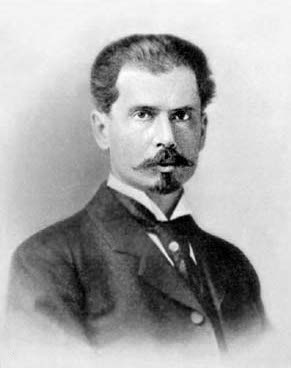
\includegraphics[width=0.26\linewidth]{images/book4/winogradsky.jpg}\hspace{0.05\linewidth}
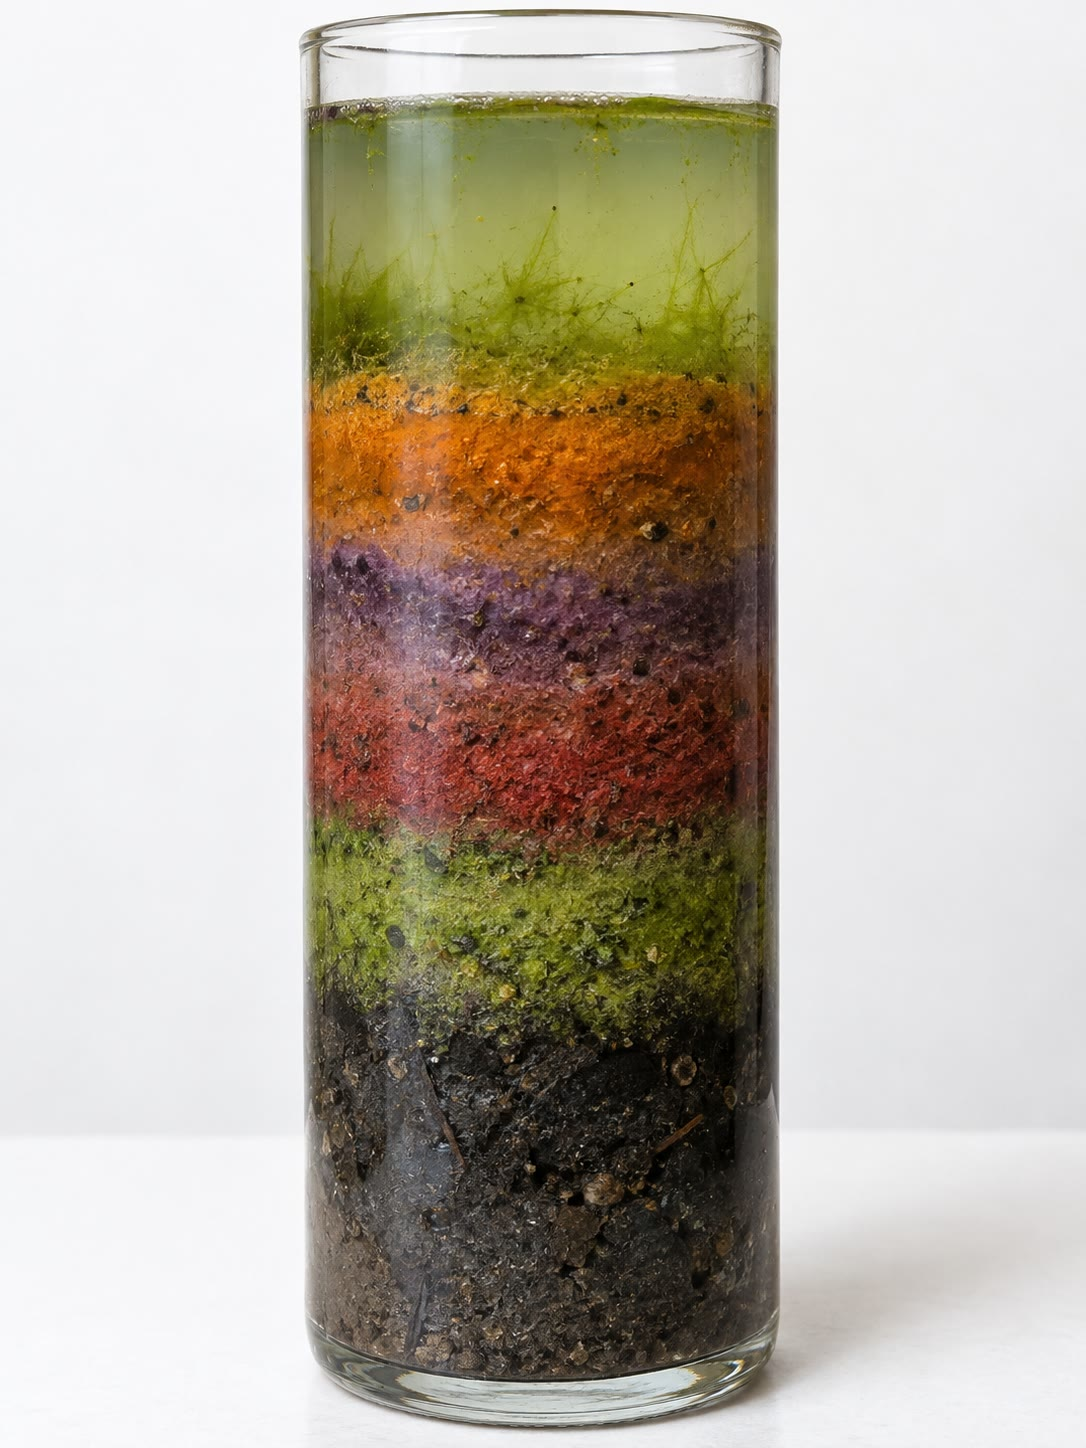
\includegraphics[width=0.30\linewidth]{images/book4/ai/b4-02-winogradsky-column.jpg}

{\small सर्गेई विनोग्रैडस्की, जिन्होंने रसशिलापोषण खोजा, और वह
बेलन जो उनका नाम धारण करता है: कीचड़ और पानी का एक बेलन जो प्रकाश में
शैवाल, लौह तथा गंधक ऑक्सीकारियों, बैंगनी और हरे गंधक-जीवाणुओं, और काली
कीचड़ में सल्फेट अपचायकों की पट्टियों में बँट जाता है।}
\end{omfigure}

\begin{definition}[अनॉक्सीजनी प्रकाशसंश्लेषण]\label{def:b2:microbial-metabolism:anoxygenic}
\index{अनॉक्सीजनी प्रकाशसंश्लेषण}
बैंगनी और हरे जीवाणु एक ही प्रकाशतंत्र और ऐसे जीवाणु-पर्णहरित से
प्रकाशसंश्लेषण करते हैं जो निकट अवरक्त में अवशोषित करता है, और जल के
बजाय $\mathrm{H_2S}$, $\mathrm{H_2}$ या कार्बनिक अम्ल इलेक्ट्रॉन दाता
के रूप में काम में लेते हैं: वे गंधक या सल्फेट छोड़ते हैं, ऑक्सीजन कभी
नहीं, और उन्हें ऐसी तरंगदैर्घ्य का प्रकाश चाहिए जो ऊपर की हरी तथा
सायनोजीवाणु परत से पार आ सके। इसीलिए बैंगनी गंधक-जीवाणु विनोग्रैडस्की
बेलन की बैंगनी पट्टी में उगते हैं, ठीक वहाँ जहाँ नीचे से आता सल्फाइड
ऊपर से आते प्रकाश से मिलता है; हरे गंधक-जीवाणु, जो अधिक सल्फाइड और कम
प्रकाश सह लेते हैं, उनके नीचे उगते हैं। ऑक्सीजनी प्रकाशसंश्लेषण, अपने
शृंखलाबद्ध दो प्रकाशतंत्रों के साथ, एक ही वंशक्रम --- सायनोजीवाणुओं ---
का बाद का आविष्कार है, जिसने जल से इलेक्ट्रॉन लेना सीखा।
\end{definition}

\section{अवायवीय श्वसन और किण्वन}

\begin{definition}[अवायवीय श्वसन]\label{def:b2:microbial-metabolism:anaerobic}
\index{अवायवीय श्वसन}\index{विनाइट्रीकरण}\index{सल्फेट अपचयन}\index{मेथेनजनन}
\emph{अवायवीय श्वसन} श्वसन ही है --- इलेक्ट्रॉन-अभिगमन शृंखला जो
प्रोटॉन पंप करती है और रसोपरासरण से ATP बनाती है --- पर ऑक्सीजन के
सिवा किसी अंतिम ग्राही के साथ। \emph{विनाइट्रीकारी}
(\emph{Pseudomonas}, \emph{Paracoccus}) नाइट्रेट को नाइट्राइट, नाइट्रिक
ऑक्साइड, नाइट्रस ऑक्साइड और अंत में $\mathrm{N_2}$ में अपचयित करते हैं,
जो वायु में निकल जाती है; वे अपनी वायवीय शृंखला ही कुछ अतिरिक्त एंजाइमों
के साथ काम में लेते हैं और नाइट्रेट पर तभी जाते हैं जब ऑक्सीजन चुक
जाए। \emph{सल्फेट अपचायक} (\emph{Desulfovibrio}) सल्फेट को सल्फाइड में
अपचयित करते हैं, कीचड़ को लौह सल्फाइड से काला कर देते हैं और उसे उसकी
गंध देते हैं। \emph{मेथेनजनक}, जो आर्किया हैं, $\mathrm{CO_2}$ को
$\mathrm{H_2}$ से मेथेन में अपचयित करते हैं ($4\mathrm{H_2} + \mathrm{CO_2} \to \mathrm{CH_4} +
2\mathrm{H_2O}$, $\Delta G^{\circ\prime} = \qty{-131}{kJ/mol}$), या
ऐसीटेट को मेथेन और $\mathrm{CO_2}$ में तोड़ते हैं; ऑक्सीजन उन्हें मार
देती है और वे गायों के रूमेन, धान के खेतों, दलदलों और कूड़ाघरों में
रहते हैं, जहाँ से वे एक हरितगृह गैस छोड़ते हैं जो
\cref{ch:b2:global-change} का विषय है। लोहे और मैंगनीज़ के ऑक्साइड और
समूहों के काम आते हैं। वर्ष 1 के खंड ने ऑक्सीजन को \emph{एकमात्र} ग्राही
माना था; पृथ्वी के अधिकांश इतिहास में, और आज हर अवसाद में, वह एक
शृंखला की केवल पहली कड़ी है।
\end{definition}

\begin{proposition}[किसी अवसाद में ग्राहियों का क्रम]\label{prop:b2:microbial-metabolism:sequence}
जलमग्न किसी अवसाद में नीचे उतरते हुए इलेक्ट्रॉन ग्राही उसी क्रम में
चुकते हैं जिस क्रम में वे ऊर्जा देते हैं: पहले कुछ मिलिमीटर में
ऑक्सीजन, फिर नाइट्रेट, फिर मैंगनीज़ और लोहे के ऑक्साइड, फिर सल्फेट, और
अंत में सबसे गहरी अनॉक्सी परत में $\mathrm{CO_2}$ (\omterm{def:b2:microbial-metabolism:anaerobic}{मेथेनजनन})। यह
क्रम मीनार का ही क्रम है: हर गहराई पर बचे हुए सर्वोत्तम ग्राही का उपयोग
करने वाले जीव सबसे तेज़ बढ़ते हैं, कार्बनिक दाताओं के लिए बाक़ी सबको
हरा देते हैं, और अगला समूह आने से पहले अपना ग्राही चुका देते हैं।
समुद्र में, जहाँ सल्फेट प्रचुर है (\qty{28}{mmol/L}), सल्फेट क्षेत्र मोटा
है और \omterm{def:b2:microbial-metabolism:anaerobic}{मेथेनजनन} कई मीटर नीचे जाकर ही आरंभ होता है; सल्फेट-दरिद्र किसी
मीठे जल के दलदल में मेथेन सतह के ठीक नीचे बनने लगती है।
\end{proposition}

\begin{omfigure}
\begin{tikzpicture}[every node/.style={font=\scriptsize}]
  \fill[omDef!8] (0,0) rectangle (4,0.6);
  \node at (2,0.3) {जल};
  \fill[omExo!35] (0,-0.5) rectangle (4,0);
  \fill[omProp!25] (0,-1.3) rectangle (4,-0.5);
  \fill[omProp!45] (0,-2.0) rectangle (4,-1.3);
  \fill[gray!50] (0,-3.4) rectangle (4,-2.0);
  \fill[black!75] (0,-4.4) rectangle (4,-3.4);
  \draw[thick] (0,0.6) -- (0,-4.4); \draw[thick] (4,0.6) -- (4,-4.4);
  \draw[thick] (0,0) -- (4,0);
  \node[anchor=west, align=left] at (4.2,-0.25) {ऑक्सीजन श्वसन: $\mathrm{O_2 \to H_2O}$ --- \qty{2.9}{MJ} प्रति ग्लूकोज़};
  \node[anchor=west, align=left] at (4.2,-0.9) {नाइट्रेट अपचयन: $\mathrm{NO_3^- \to N_2}$ --- \qty{2.7}{MJ}};
  \node[anchor=west, align=left] at (4.2,-1.65) {मैंगनीज़ और लौह अपचयन: $\mathrm{Fe^{3+} \to Fe^{2+}}$};
  \node[anchor=west, align=left, white] at (0.1,-2.7) {};
  \node[anchor=west, align=left] at (4.2,-2.7) {सल्फेट अपचयन: $\mathrm{SO_4^{2-} \to H_2S}$ --- \qty{0.5}{MJ}};
  \node[anchor=west, align=left] at (4.2,-3.9) {मेथेनजनन: $\mathrm{CO_2 \to CH_4}$ --- \qty{0.4}{MJ}};
  \draw[->, thick] (-0.5,0) -- (-0.5,-4.4) node[below] {गहराई};
  \node[anchor=east] at (-0.6,-0.25) {mm};
  \node[anchor=east] at (-0.6,-2.7) {सेमी से मी};
\end{tikzpicture}

{\small किसी अवसाद में गहराई के साथ इलेक्ट्रॉन ग्राहियों का अनुक्रम,
प्रति ग्लूकोज़ मिलने वाली ऊर्जा के क्रम में। हर क्षेत्र के जीव कार्बनिक
पदार्थ के लिए अगले क्षेत्र को तब तक हराते रहते हैं जब तक उनका ग्राही चुक
न जाए।}
\end{omfigure}

\begin{definition}[किण्वन, फिर से]\label{def:b2:microbial-metabolism:fermentation}
\index{किण्वन!सूक्ष्मजैविक}
\emph{किण्वन} कोई बाहरी ग्राही काम में नहीं लेता: कार्बनिक क्रियाधार
एक अधिक ऑक्सीकृत और एक अधिक अपचयित उत्पाद में बँट जाता है, ATP केवल
क्रियाधार-स्तरीय फ़ॉस्फ़ोरिलीकरण से बनती है, और ग्लाइकोलिसिस की NADH
किसी उपापचयज को अपचयित करके फिर ऑक्सीकृत हो जाती है। खमीर एथेनॉल और
$\mathrm{CO_2}$ बनाते हैं; लैक्टिक जीवाणु लैक्टेट बनाते हैं (दही,
साउरक्राउट, दुखती पेशियाँ); \emph{E.~coli} अम्लों, एथेनॉल और गैसों का
मिश्रण बनाता है; क्लॉस्ट्रिडिया ब्यूटिरेट, ब्यूटेनॉल और ऐसीटोन बनाते
हैं; प्रोपिओनिजीवाणु स्विस पनीर का प्रोपिओनेट और $\mathrm{CO_2}$ बनाते
हैं। उपज श्वसन के कोई तीस के मुक़ाबले दो ATP प्रति ग्लूकोज़ है, इसलिए
किण्वकारी को उतनी ही वृद्धि के लिए पंद्रह गुना अधिक शर्करा निपटानी पड़ती
है, और उसके उत्पाद --- अम्ल, ऐल्कोहॉल --- उसके अपने ही माध्यम को
विषैला कर देते हैं: किण्वन भोजन को इसीलिए सुरक्षित रखता है कि किण्वकारी
भोजन को रहने लायक़ नहीं छोड़ता, अपने लिए भी नहीं।
\end{definition}

\begin{example}[सहभोजिता: बचे-खुचे पर जीना]\label{ex:b2:microbial-metabolism:syntrophy}
किसी अनॉक्सी अवसाद में किण्वकारी पीछे ऐसीटेट, प्रोपिओनेट, ब्यूटिरेट और
$\mathrm{H_2}$ छोड़ जाते हैं। प्रोपिओनेट को ऐसीटेट और
$\mathrm{H_2}$ में ऑक्सीकृत करने की मानक मुक्त ऊर्जा \emph{धनात्मक}
(\qty{+76}{kJ/mol}) है और वह असंभव है --- जब तक पड़ोस का कोई मेथेनजनक
हाइड्रोजन को उतनी ही तेज़ी से न खाता रहे जितनी तेज़ी से वह बनती है, और
उसका आंशिक दाब \qty{1e-4}{atm} से नीचे न रखे, जिस पर वह अभिक्रिया
ऊर्जादायी हो जाती है। दोनों में से कोई भी साथी प्रोपिओनेट पर अकेले नहीं
बढ़ सकता; साथ मिलकर वे उसे मेथेन बना देते हैं। यही \emph{अंतरजातीय
हाइड्रोजन हस्तांतरण} कारण है कि अवायवीय पाचन सदा किसी संघ का काम होता
है, और कि वह आर्किया तथा उसका जीवाणु साथी प्रायः एक-दूसरे से सटे हुए
मिलते हैं।
\end{example}

\section{किसी क्रियाधार पर वृद्धि}

\begin{theorem}[मोनो का नियम]\label{thm:b2:microbial-metabolism:monod}
\index{मोनो समीकरण}\index{उपज गुणांक}
$S$ सांद्रता के किसी एकल सीमाकारी क्रियाधार पर बढ़ती किसी आबादी की
विशिष्ट वृद्धि दर है
\[
\mu = \mu_{\max}\,\frac{S}{K_s + S}, \qquad \frac{\mathrm{d}X}{\mathrm{d}t} = \mu X,
\]
जिसमें $X$ जैवभार सांद्रता है, $\mu_{\max}$ अधिकतम दर (सबसे छोटे
\omterm{def:b2:unicellular-diversity:division}{पीढ़ी काल} का व्युत्क्रम, $\ln 2$ से भाग देकर) और $K_s$
\emph{अर्ध-संतृप्ति स्थिरांक}, यानी वह क्रियाधार सांद्रता जिस पर वृद्धि
आधी चाल से चलती है --- \emph{E.~coli} के लिए ग्लूकोज़ के कुछ मिलिग्राम
प्रति लीटर। क्रियाधार वृद्धि के समानुपात में खपता है,
$\mathrm{d}S/\mathrm{d}t =
-\mu X/Y$, जिसमें $Y$ \emph{उपज} है: प्रति ग्राम क्रियाधार जितने ग्राम
जैवभार, शर्करा पर वायवीय वृद्धि के लिए लगभग \num{0.5} और किसी
किण्वकारी के लिए \num{0.1}।
\end{theorem}
\begin{proof}[प्रमाण-सामग्री]
मोनो (1942) ने \emph{E.~coli} को ग्लूकोज़ की अनेक सांद्रताओं पर बैचों
में उगाया और हर एक की चरघातांकी दर मापी: दरें सांद्रता के साथ चढ़ीं और
माइकेलिस--मेंटन वक्र की तरह संतृप्त हो गईं, जो ठीक वही अपेक्षित है जब दर
किसी संतृप्त हो सकने वाले ग्रहण तंत्र से तय होती हो। यह नियम आनुभविक है
--- कोशिका में हज़ारों एंजाइम हैं, एक नहीं --- पर वह लगभग हर
क्रियाधार-सीमित संवर्धन पर ठीक बैठता है, और वह \omterm{def:b2:microbial-metabolism:fermentation}{किण्वन} प्रौद्योगिकी
तथा अपजल अभियांत्रिकी की नींव है।
\end{proof}

\begin{theorem}[केमोस्टैट]\label{thm:b2:microbial-metabolism:chemostat}
\index{केमोस्टैट}\index{तनुकरण दर}
\emph{केमोस्टैट} $V$ आयतन का ऐसा पात्र है जिसे ताज़ा माध्यम (क्रियाधार
$S_{\mathrm{in}}$) $F$ प्रवाह पर पिलाया जाता है और उसी प्रवाह पर निथारा
जाता है, ताकि \emph{\omterm{thm:b2:microbial-metabolism:chemostat}{तनुकरण दर}} $D = F/V$ हो। जैवभार और
क्रियाधार इनका पालन करते हैं:
\[
\frac{\mathrm{d}X}{\mathrm{d}t} = (\mu - D)\,X, \qquad
\frac{\mathrm{d}S}{\mathrm{d}t} = D\,(S_{\mathrm{in}} - S) - \frac{\mu X}{Y}.
\]
स्थायी अवस्था में $\mu = D$: संवर्धन ठीक उतनी ही तेज़ी से बढ़ता है जितनी
तेज़ी से वह बहाया जाता है, किसी क्रांतिक मान से नीचे के किसी भी $D$ के
लिए, और संचालक पंप घुमाकर वृद्धि दर तय कर देता है। स्थायी अवस्था के
क्रियाधार और जैवभार ये हैं:
\[
S^* = \frac{K_s\,D}{\mu_{\max} - D}, \qquad X^* = Y\,(S_{\mathrm{in}} - S^*),
\]
और \emph{बहाव} दर $D_c = \mu_{\max}
S_{\mathrm{in}}/(K_s + S_{\mathrm{in}})$ से ऊपर कोई आबादी टिक नहीं सकती।
\end{theorem}
\begin{proof}
$\mathrm{d}X/\mathrm{d}t = 0$ को $X \neq 0$ के साथ रखने पर $\mu = D$ मिलता है;
मोनो का नियम उलटने पर $D(K_s + S^*) = \mu_{\max} S^*$, इसलिए $S^* =
K_s D/(\mu_{\max} - D)$। $\mathrm{d}S/\mathrm{d}t = 0$ रखकर और $\mu$ की
जगह $D$ रखने पर: $D(S_{\mathrm{in}} - S^*) = DX^*/Y$, इसलिए
$X^*$ मिलता है। हल तभी तक है जब तक $S^* < S_{\mathrm{in}}$, यानी
$D < \mu_{\max} S_{\mathrm{in}}/(K_s + S_{\mathrm{in}})$; उससे आगे $\mu < D$ है,
हर $S \le S_{\mathrm{in}}$ के लिए, और $X$ घटकर शून्य हो जाता है।
यह स्थायी अवस्था स्थिर है: $X$ चढ़े तो $S$ गिरता है, $\mu$ $D$ से नीचे
आता है और $X$ फिर बहकर नीचे आ जाता है।
\end{proof}

\begin{omfigure}
\begin{minipage}[b]{0.48\linewidth}\centering
\begin{tikzpicture}
\begin{axis}[
  width=0.94\linewidth, height=5.4cm,
  axis x line=bottom, axis y line=left,
  xmin=0, xmax=0.5, ymin=0, ymax=1.1,
  xlabel={$S$ (\unit{g/L})}, ylabel={$\mu$ (\unit{h^{-1}})},
  xlabel style={font=\small, at={(axis description cs:0.5,-0.14)}, anchor=north},
  ylabel style={font=\small},
  tick label style={font=\small}, xtick={0,0.1,0.2,0.3,0.4,0.5}, ytick={0,0.5,1},
  clip=false,
]
\addplot[very thick, omDef, domain=0:0.5, samples=100] {x/(0.02+x)};
\draw[dashed, gray] (axis cs:0,1) -- (axis cs:0.5,1); \node[font=\scriptsize, anchor=south east] at (axis cs:0.5,1) {$\mu_{\max}$};
\draw[dashed, gray] (axis cs:0,0.5) -- (axis cs:0.02,0.5) -- (axis cs:0.02,0); \node[font=\scriptsize, anchor=north west] at (axis cs:0.02,-0.02) {$K_s$};
\end{axis}
\end{tikzpicture}
\end{minipage}\hfill
\begin{minipage}[b]{0.5\linewidth}\centering
\begin{tikzpicture}
\begin{axis}[
  width=0.94\linewidth, height=5.4cm,
  axis x line=bottom, axis y line=left,
  xmin=0, xmax=1.1, ymin=0, ymax=2.2,
  xlabel={तनुकरण दर $D$ (\unit{h^{-1}})}, ylabel={\unit{g/L}},
  xlabel style={font=\small, at={(axis description cs:0.5,-0.14)}, anchor=north},
  ylabel style={font=\small},
  tick label style={font=\small}, xtick={0,0.5,1}, ytick={0,1,2},
  legend style={font=\scriptsize, at={(0.05,0.62)}, anchor=west, draw=none},
  clip=false,
]
\addplot[very thick, omDef, domain=0:0.99, samples=200] {0.5*(2 - 0.02*x/(1-x))};
\addlegendentry{जैवभार $X^*$}
\addplot[very thick, omThm, domain=0:0.99, samples=200] {0.02*x/(1-x)};
\addlegendentry{क्रियाधार $S^*$}
\addplot[thick, omProp, dashed, domain=0:0.99, samples=200] {x*0.5*(2 - 0.02*x/(1-x))};
\addlegendentry{निर्गत $D X^*$}
\draw[dashed, gray] (axis cs:0.99,0) -- (axis cs:0.99,2.1); \node[font=\scriptsize, anchor=south, align=center] at (axis cs:0.9,2.1) {बहाव};
\end{axis}
\end{tikzpicture}
\end{minipage}

{\small बाएँ: $\mu_{\max} = \qty{1}{h^{-1}}$ और
$K_s = \qty{0.02}{g/L}$ के साथ मोनो का नियम। दाएँ: \qty{2}{g/L}
क्रियाधार पिलाया गया केमोस्टैट ($Y = 0.5$): बहाव दर तक जैवभार लगभग
अचर रहता है और अवशिष्ट क्रियाधार लगभग शून्य, और उस दर के पास
क्रियाधार फूट निकलता है तथा आबादी ढह जाती है; प्रति घंटा जैवभार
निर्गत ठीक उससे पहले सबसे अधिक होता है।}
\end{omfigure}

\begin{omfigure}
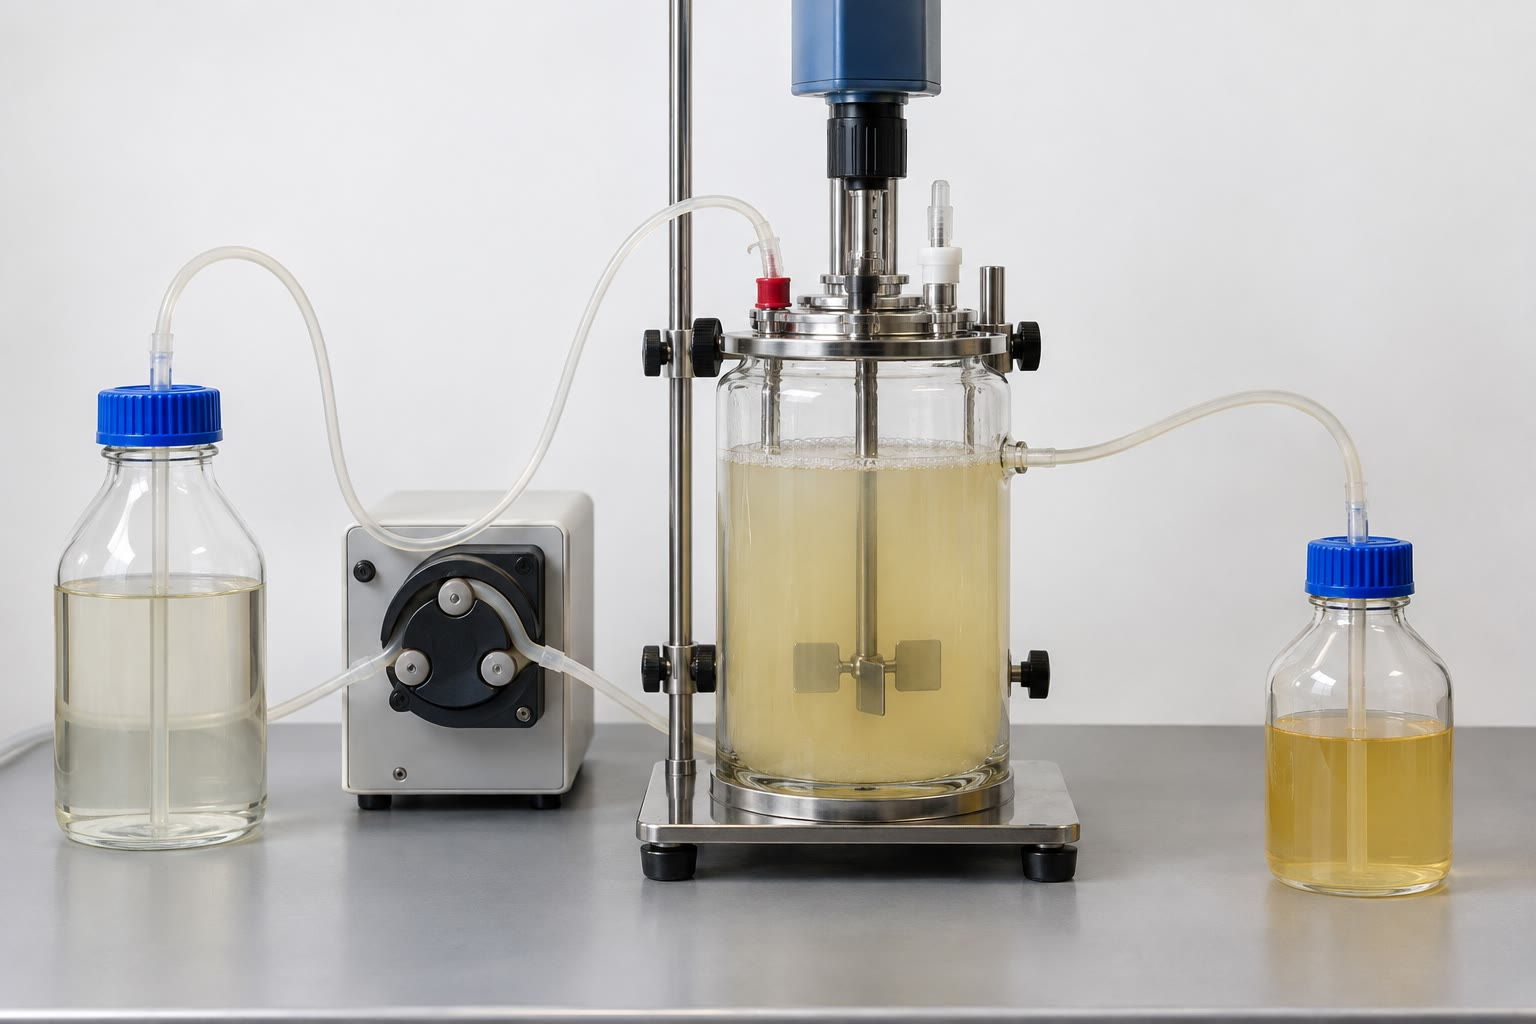
\includegraphics[width=0.6\linewidth]{images/book4/ai/b4-02-chemostat.jpg}

{\small प्रयोगशाला का एक केमोस्टैट: बाईं ओर के भंडार से ताज़ा माध्यम
पंप किया जाता है, संवर्धन दाईं ओर उफनकर निकलता है; पंप ही वृद्धि दर तय
करता है।}
\end{omfigure}

\begin{example}[किसी केमोस्टैट को पढ़ना]\label{ex:b2:microbial-metabolism:chemostat}
$\mu_{\max} = \qty{1.0}{h^{-1}}$, $K_s = \qty{0.02}{g/L}$,
$S_{\mathrm{in}} = \qty{2}{g/L}$ और $Y = 0.5$ के साथ, $D =
\qty{0.5}{h^{-1}}$ पर: $S^* = 0.02\times 0.5/0.5 = \qty{0.02}{g/L}$ और
$X^* = 0.5\times 1.98 = \qty{0.99}{g/L}$; संवर्धन शर्करा का
\qty{1}{\%} अनछुआ छोड़ देता है। बहाव दर $1.0\times
2/2.02 = \qty{0.99}{h^{-1}}$ है। कोई पाचक या कोई आँत इसी सिद्धांत पर
चलती है: मानव बृहदांत्र, जिसे दिन में तीन बार भरा और एक बार ख़ाली किया
जाता है, अपने जीवाणुओं को \qty{0.04}{h^{-1}} के पास की \omterm{thm:b2:microbial-metabolism:chemostat}{तनुकरण दर} पर रखती है, और जो
जाति एक दिन में दुगुनी नहीं हो सकती वह बह जाती है --- जब तक वह भित्ति
से चिपक न जाए।
\end{example}

\section{जैवफ़िल्में}

\begin{definition}[जैवफ़िल्म]\label{def:b2:microbial-metabolism:biofilm}
\index{जैवफ़िल्म}\index{बाह्यकोशिकीय आधात्री!जीवाणुओं की}
\emph{जैवफ़िल्म} सूक्ष्मजीवों का ऐसा समुदाय है जो किसी सतह से जुड़ा
होता है और स्वयं बनाई \emph{आधात्री} में --- बहुशर्कराओं, प्रोटीनों और
बाह्यकोशिकीय DNA की --- धँसा रहता है। वह चरणों में बनती है: अकेली
कोशिकाओं का प्रतिवर्ती \emph{संलग्नन} (कशाभ, पिली), अप्रतिवर्ती संलग्नन
और \emph{सूक्ष्मनिवह} वृद्धि, मीनारों तथा जल-नलिकाओं वाली संरचित फ़िल्म
में \emph{परिपक्वन}, और उन कोशिकाओं का \emph{प्रकीर्णन} जो तैरकर नई
सतहें बसाने निकल जाती हैं। आधात्री जल और पोषक थामे रखती है, कोशिकाओं को
निर्जलीकरण, चरने वालों, प्रतिजैविकों और प्रतिरक्षा कोशिकाओं से बचाती है,
और ऐसी रासायनिक प्रवणताएँ खड़ी करती है जो उस फ़िल्म को निकेतों का
भूदृश्य बना देती हैं। पृथ्वी के अधिकांश जीवाणु ऐसे ही जीते हैं: धाराओं
की चट्टानों पर, जड़ों पर, दाँतों पर (दंत पट्टिका), कैथेटरों और
प्रत्यारोपों पर, सिस्टिक फ़ाइब्रोसिस के रोगियों के फेफड़ों में, जहाज़ों
के पेंदों पर और पाइपों में।
\end{definition}

\begin{omfigure}
\begin{tikzpicture}[every node/.style={font=\scriptsize}]
  \fill[gray!35] (0,0) rectangle (13.6,0.35);
  \node at (6.8,0.17) {सतह};
  % stage 1 attachment
  \foreach \p in {(0.6,0.55),(1.4,0.55)} \draw[thick, omDef, fill=omDef!30] \p ellipse (0.22 and 0.1);
  \draw[thick, omDef, fill=omDef!30] (1.0,1.6) ellipse (0.22 and 0.1);
  \draw[->, omDef] (1.0,1.45) -- (1.0,0.75);
  \node[below, align=center] at (1.1,-0.05) {1. संलग्नन};
  % stage 2 microcolony
  \begin{scope}[xshift=3.4cm]
    \fill[omExo!25] (0.15,0.35) .. controls (0.1,1.1) and (1.5,1.1) .. (1.45,0.35);
    \foreach \p in {(0.45,0.5),(0.8,0.5),(1.15,0.5),(0.6,0.75),(0.95,0.75),(0.8,0.95)} \draw[thick, omDef, fill=omDef!30] \p ellipse (0.18 and 0.09);
    \node[below, align=center] at (0.8,-0.05) {2. सूक्ष्मनिवह,\\आधात्री स्राव};
  \end{scope}
  % stage 3 mature with channels
  \begin{scope}[xshift=6.8cm]
    \fill[omExo!25] (0.0,0.35) .. controls (0.2,1.9) and (0.9,2.2) .. (1.1,1.5) .. controls (1.2,0.9) and (1.4,0.6) .. (1.5,0.35);
    \fill[omExo!25] (1.7,0.35) .. controls (1.6,1.5) and (2.6,2.3) .. (2.9,1.2) .. controls (3.0,0.8) and (3.1,0.5) .. (3.2,0.35);
    \foreach \p in {(0.35,0.55),(0.7,0.55),(0.5,0.85),(0.8,1.15),(0.55,1.45),(2.0,0.6),(2.4,0.6),(2.2,0.9),(2.5,1.25),(2.3,1.6),(2.6,1.9),(2.1,1.3)} \draw[thick, omDef, fill=omDef!30] \p ellipse (0.16 and 0.08);
    \draw[<->, omThm, thick] (1.6,0.5) -- (1.6,1.6);
    \node[omThm, anchor=south] at (1.6,2.45) {जल-नलिका};
    \node[below, align=center] at (1.6,-0.05) {3. परिपक्व फ़िल्म: मीनारें,\\नलिकाएँ, प्रवणताएँ};
  \end{scope}
  % stage 4 dispersal
  \begin{scope}[xshift=11.2cm]
    \fill[omExo!25] (0.0,0.35) .. controls (0.1,1.5) and (1.0,1.6) .. (1.1,0.35);
    \foreach \p in {(0.3,0.55),(0.65,0.55),(0.5,0.85)} \draw[thick, omDef, fill=omDef!30] \p ellipse (0.16 and 0.08);
    \foreach \p/\a in {(1.4,1.5)/40,(1.9,1.1)/10,(1.6,2.0)/70} \draw[thick, omDef, fill=omDef!30, rotate around={\a:\p}] \p ellipse (0.16 and 0.08);
    \draw[->, omDef] (1.0,1.0) -- (1.35,1.35);
    \node[below, align=center] at (1.0,-0.05) {4. प्रकीर्णन};
  \end{scope}
\end{tikzpicture}

{\small किसी \omterm{def:b2:microbial-metabolism:biofilm}{जैवफ़िल्म} का जीवन-चक्र: अकेली कोशिकाएँ जुड़ती हैं, बढ़कर
ऐसे सूक्ष्मनिवह बनती हैं जो एक आधात्री (धूसर) स्रावित करते हैं, मीनारों
और जल-नलिकाओं वाली संरचित फ़िल्म में परिपक्व होती हैं, और तैरती कोशिकाएँ
छोड़ती हैं जो नई सतहें बसाती हैं।}
\end{omfigure}

\begin{omfigure}
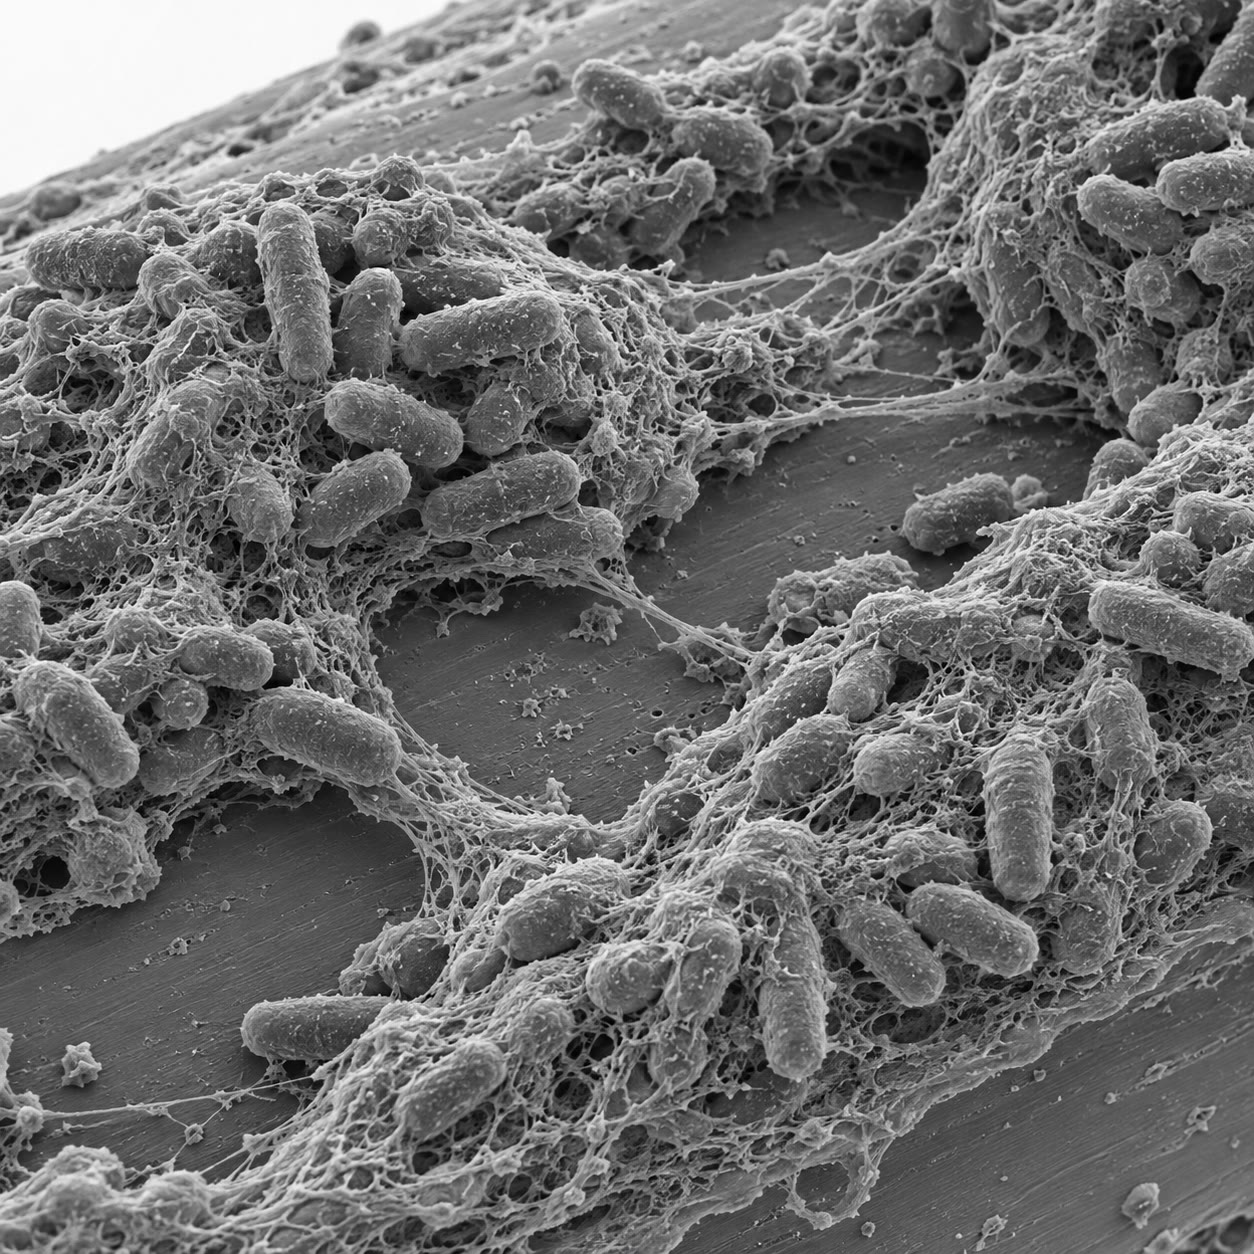
\includegraphics[width=0.46\linewidth]{images/book4/ai/b4-02-biofilm-sem.jpg}

{\small किसी कैथेटर पर एक \omterm{def:b2:microbial-metabolism:biofilm}{जैवफ़िल्म}, क्रमवीक्षी इलेक्ट्रॉन
सूक्ष्मदर्शन में: छड़-आकार के जीवाणु उसी तंतुमय आधात्री में धँसे हैं जो
उन्होंने स्रावित की है, और गुच्छों के बीच खुली नलिकाएँ हैं।}
\end{omfigure}

\begin{theorem}[किसी जैवफ़िल्म के भीतर प्रवणताएँ]\label{thm:b2:microbial-metabolism:gradient}
\index{ऑक्सीजन प्रवेश गहराई}
$L$ मोटाई की किसी ऐसी फ़िल्म में जिसकी कोशिकाएँ अचर आयतनी दर $q$ से
ऑक्सीजन खपाती हैं, जिसकी सतह पर सांद्रता $c_0$ बनी रहती है और जिसके
आधार से कोई अभिवाह नहीं, स्थायी अवस्था का ऑक्सीजन परिच्छेद एक परवलय है,
और यदि फ़िल्म इतनी मोटी हो कि ऑक्सीजन चुक जाए, तो वह \emph{प्रवेश
गहराई} पर चुकती है:
\[
L_p = \sqrt{\frac{2 D_e\, c_0}{q}},
\]
जिसमें $D_e$ आधात्री में प्रभावी विसरण गुणांक है।
$D_e = \qty{1.5e-9}{m^2/s}$, $c_0 = \qty{0.25}{mol/m^3}$ और $q
= \qty{0.17}{mol/m^3/s}$ (श्वसनरत कोशिकाओं की सघन फ़िल्म) के साथ $L_p
\approx \qty{66}{\micro m}$: मिलिमीटर के दसवें भाग से नीचे कोई \omterm{def:b2:microbial-metabolism:biofilm}{जैवफ़िल्म}
अनॉक्सी होती है, और विनाइट्रीकारी, किण्वकारी तथा सल्फेट अपचायक
वायुजीवियों की छत के नीचे रहते हैं।
\end{theorem}
\begin{proof}
मान लीजिए $x$ सतह से नीचे की गहराई है। स्थायी अवस्था में विसरण अभिवाह
$-D_e\,\mathrm{d}c/\mathrm{d}x$ गहराई के साथ केवल खपत से बदलता है:
$D_e\,\mathrm{d}^2c/\mathrm{d}x^2 = q$। दो बार समाकलन करने पर
$c = c_0 + a x + q x^2/2D_e$। यदि ऑक्सीजन $L_p$ गहराई पर, वहाँ शून्य
अभिवाह के साथ (नीचे से कुछ नहीं आता), लुप्त हो जाए, तो
$c(L_p) = 0$ और $c'(L_p) = 0$: दूसरे से $a = -qL_p/D_e$ मिलता है,
और तब पहले से $c_0 - qL_p^2/D_e + qL_p^2/2D_e = 0$, यानी
$L_p^2 = 2D_e c_0/q$। परिच्छेद $c = (q/2D_e)(L_p - x)^2$ है।
\end{proof}

\begin{omfigure}
\begin{tikzpicture}
\begin{axis}[
  width=0.78\linewidth, height=5.6cm,
  axis x line=bottom, axis y line=left,
  xmin=0, xmax=120, ymin=0, ymax=0.28,
  xlabel={फ़िल्म में गहराई (\unit{\micro m})}, ylabel={$\mathrm{O_2}$ (\unit{mol/m^3})},
  xlabel style={font=\small, at={(axis description cs:0.5,-0.14)}, anchor=north},
  ylabel style={font=\small},
  tick label style={font=\small}, xtick={0,20,40,60,80,100,120}, ytick={0,0.1,0.2},
  clip=false,
]
\addplot[very thick, omDef, domain=0:66, samples=60] {0.25*(1-x/66)^2};
\addplot[very thick, omDef, domain=66:120, samples=2] {0};
\fill[omThm!12] (axis cs:66,0) rectangle (axis cs:120,0.28);
\node[font=\scriptsize, anchor=north, align=center] at (axis cs:93,0.27) {अनॉक्सी क्षेत्र:\\विनाइट्रीकारी, किण्वकारी,\\सल्फेट अपचायक};
\draw[dashed, gray] (axis cs:66,0) -- (axis cs:66,0.28); \node[font=\scriptsize, anchor=south] at (axis cs:66,0.28) {$L_p$};
\node[font=\scriptsize, anchor=west] at (axis cs:24,0.18) {वायवीय क्षेत्र};
\end{axis}
\end{tikzpicture}

{\small श्वसनरत किसी \omterm{def:b2:microbial-metabolism:biofilm}{जैवफ़िल्म} के भीतर ऑक्सीजन: सतह पर के थोक मान से
प्रवेश गहराई पर शून्य तक परवलयी गिरावट, जो प्रमेय के आँकड़ों के लिए
\qty{66}{\micro m} है। इससे गहरा सब कुछ अनॉक्सी है।}
\end{omfigure}

\begin{proposition}[कोरम संवेदन]\label{prop:b2:microbial-metabolism:quorum}
\index{कोरम संवेदन}\index{स्वप्रेरक}
जीवाणु अपनी गिनती करते हैं। हर कोशिका एक छोटा संकेत-अणु, कोई
\emph{स्वप्रेरक} (ग्राम-ऋणियों में ऐसिल-होमोसिरीन लैक्टोन,
ग्राम-धनियों में छोटे पेप्टाइड), कम अचर दर से स्रावित करती है। किसी तनु
निलंबन में वह संकेत विसरित होकर उड़ जाता है; किसी सघन आबादी या
\omterm{def:b2:microbial-metabolism:biofilm}{जैवफ़िल्म} में वह जमा होता है, और किसी देहली सांद्रता से ऊपर वह किसी
ग्राही से बँधकर जीनों का एक समुच्चय चालू कर देता है --- जिनमें स्वप्रेरक
का अपना जीन भी है, और नाम यहीं से आया है। यों नियंत्रित जीन वे हैं जो
तभी फल देते हैं जब अनेक कोशिकाएँ मिलकर काम करें: दीप्ति, पाचक एंजाइमों
तथा विषों का स्राव, आधात्री का उत्पादन, उन रोगजनकों की उग्रता जिन्हें
पोषी पर एक साथ टूट पड़ना है, न कि एक-एक कोशिका करके उसे सचेत करना।
\end{proposition}
\begin{proof}[प्रमाण-सामग्री]
नील्सन, प्लैट और हेस्टिंग्स (1970) ने पाया कि समुद्री जीवाणु
\emph{Vibrio fischeri}, जो किसी स्क्विड का अंग जगमगाता है, तनु संवर्धन
में अंधकारमय रहता है और प्रति मिलिलिटर लगभग $10^{7}$ कोशिकाओं से ऊपर ही
चमकता है; किसी सघन, चमकते संवर्धन से लिया कोशिका-रहित माध्यम किसी तनु
संवर्धन को तुरंत चमका देता था। उस माध्यम में वह संकेत था; उसकी संरचना,
एक ऐसिल-होमोसिरीन लैक्टोन, 1981 में तय हुई, और जो उत्परिवर्ती उसे बना
नहीं सकते वे कितने भी सघन हो जाएँ, कभी नहीं चमकते।
\end{proof}

\begin{example}[कोई जैवफ़िल्म प्रतिजैविकों से क्यों बच जाती है]\label{ex:b2:microbial-metabolism:tolerance}
किसी \omterm{def:b2:microbial-metabolism:biofilm}{जैवफ़िल्म} की कोशिकाएँ प्रतिजैविक की उन सांद्रताओं से सौ से हज़ार
गुना अधिक सह लेती हैं जो उसी विभेद को निलंबन में मार डालती हैं, और वह
भी बिना किसी प्रतिरोध जीन के। आधात्री औषधि का विसरण धीमा करती है और
उसका कुछ भाग बाँध लेती है; प्रवणताएँ गहरी कोशिकाओं को भूखा, अनॉक्सी और
बमुश्किल बढ़ता छोड़ देती हैं, और अधिकांश प्रतिजैविक केवल बढ़ती कोशिकाएँ
मारते हैं (पेनिसिलिनों को भित्ति संश्लेषण चाहिए, ऐमीनोग्लाइकोसाइडों को
सक्रिय अभिगमन); कुछ \emph{अड़ियल} कोशिकाएँ तो पूरी तरह प्रसुप्त रहती हैं
और उपचार रुकते ही फ़िल्म फिर उगा देती हैं। इसलिए किसी प्रत्यारोप पर के
चिरकालिक संक्रमण का उपचार प्रायः प्रत्यारोप निकालकर ही किया जाता है।
\end{example}

\section{सूक्ष्मजैविक समुदाय}

\begin{example}[विनोग्रैडस्की बेलन, समझाया हुआ]\label{ex:b2:microbial-metabolism:column}
प्रकाश और वायु ऊपर से आते हैं; कार्बनिक पदार्थ और सल्फेट कीचड़ से।
सायनोजीवाणु और शैवाल ऊपर उगते हैं और ऑक्सीजन छोड़ते हैं। उनके नीचे
परपोषी कार्बनिक पदार्थ पर ऑक्सीजन चुका देते हैं, फिर नाइट्रेट; और गहरे,
सल्फेट अपचायक सल्फेट को सल्फाइड में बदलते हैं, जो ऊपर की ओर विसरित होकर
कीचड़ को लौह सल्फाइड से काला कर देता है। जहाँ चढ़ता सल्फाइड उतरते प्रकाश
से मिलता है, वहाँ बैंगनी गंधक-जीवाणु उसे प्रकाशसंश्लेषी ढंग से ऑक्सीकृत
करते हैं (बैंगनी पट्टी), और उनके नीचे हरे गंधक-जीवाणु; जहाँ सल्फाइड
ऑक्सीजन से मिलता है, अँधेरे में, वहाँ \emph{Beggiatoa} जैसे रंगहीन
गंधक-ऑक्सीकारी \omterm{def:b2:microbial-metabolism:trophic}{रसशिलापोषी} ढंग से जीविका कमाते हैं (सफ़ेद परदा); और जहाँ
अपचयित लोहा ऑक्सीजन से मिलता है, वहाँ लौह ऑक्सीकारी ज़ंग-रंगी पट्टी
छोड़ जाते हैं। गंधक बेलन के भीतर ही सल्फाइड और सल्फेट के बीच चक्कर काटता
है; कार्बन $\mathrm{CO_2}$ और कार्बनिक पदार्थ के बीच; केवल प्रकाश भीतर
आता है और केवल ऊष्मा बाहर जाती है। यह खुले ऊर्जा-बजट वाला एक बंद
पारितंत्र है, और समुद्र-तल का एक नमूना-प्रतिरूप।
\end{example}

\begin{omfigure}
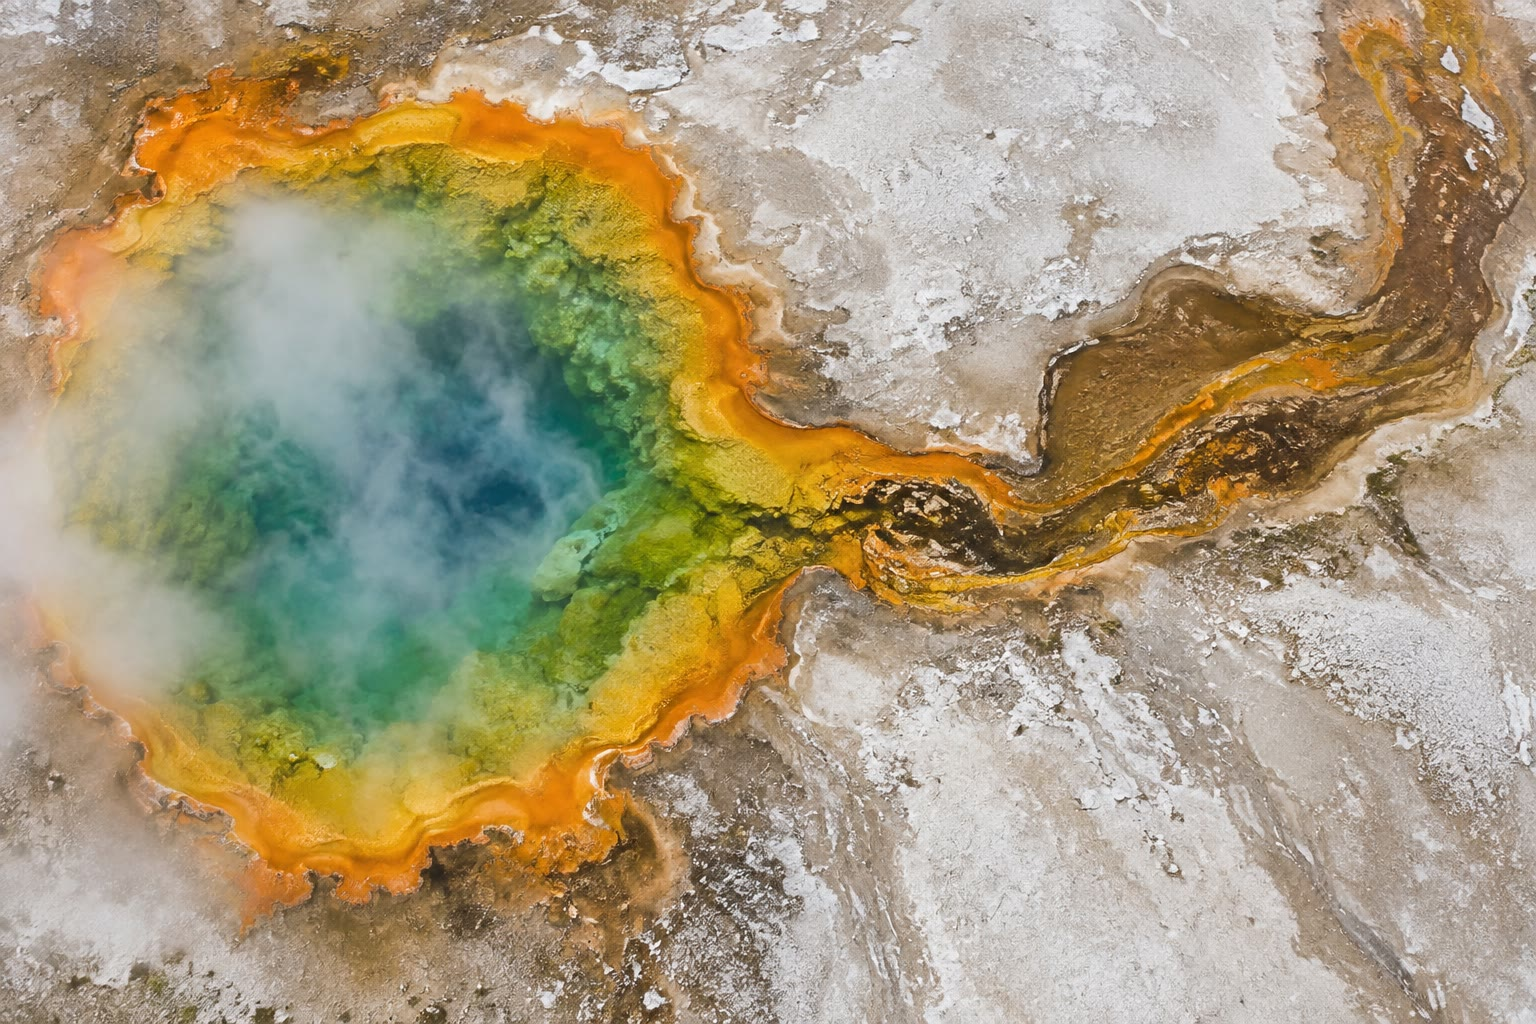
\includegraphics[width=0.62\linewidth]{images/book4/ai/b4-02-hot-spring-mats.jpg}

{\small किसी गर्म जल-स्रोत के चारों ओर सूक्ष्मजैविक चटाइयाँ: हर रंग एक
आबादी है जो अपनी पट्टी के ताप और रसायन पर जीती है --- ठंडे बहाव में
तापरागी सायनोजीवाणु और हरे जीवाणु, सबसे गर्म जल में रंगहीन
\omterm{def:b2:microbial-metabolism:trophic}{रसशिलापोषी}।}
\end{omfigure}

\begin{remark}[सूक्ष्मजैविक चटाइयाँ और आरंभिक पृथ्वी]\label{rem:b2:microbial-metabolism:mats}
गर्म जल-स्रोतों के आसपास और ज्वारीय समतलों पर, कुछ मिलिमीटर मोटी स्तरित
सूक्ष्मजैविक चटाइयाँ पूरे बेलन को उतनी मोटाई में समेट देती हैं जिसे
प्रकाश पार कर सके: ऊपर सायनोजीवाणु, उनके नीचे बैंगनी जीवाणु, आधार पर
सल्फेट अपचायक, हर परत वही खाती है जो उसके ऊपर वाली बनाती है, और वह चटाई
अपने फँसाए अवसाद में से ऊपर खिसकती रहती है। जीवाश्म चटाइयाँ ---
स्ट्रोमैटोलाइट --- जीवन के सबसे पुराने प्रमाण हैं, \num{3.5} अरब वर्ष
पुराने। दो अरब वर्षों तक, पौधों या प्राणियों से पहले, जीवमंडल यही
चटाइयाँ और उनके ऊपर का प्लवक था, और उन्हीं ने वायु को ऑक्सीजन से भरा
(\cref{ch:b2:biogeochemical-cycles})।
\end{remark}

\section{अभ्यास}

\begin{exercise}[$\star$]\label{exo:b2:microbial-metabolism:1}
ऊर्जा स्रोत, इलेक्ट्रॉन स्रोत और कार्बन स्रोत के अनुसार वर्गीकृत कीजिए:
कोई सायनोजीवाणु; \emph{Nitrosomonas}; ग्लूकोज़ पर \emph{E.~coli};
सक्सिनेट पर प्रकाश में बढ़ता कोई बैंगनी अ-गंधक जीवाणु; अँधेरे में
$\mathrm{H_2S}$ पर \emph{Thiobacillus}।
\end{exercise}

\begin{exercise}[$\star$]\label{exo:b2:microbial-metabolism:2}
श्वसन के इलेक्ट्रॉन ग्राहियों को घटती ऊर्जा-उपज के क्रम में सूचीबद्ध
कीजिए, और बताइए कि किसी अवसाद में हर एक कहाँ काम आता है।
\end{exercise}

\begin{exercise}[$\star$]\label{exo:b2:microbial-metabolism:3}
ग्लूकोज़ के $\mathrm{CO_2}$ तक ऑक्सीकरण को नाइट्रेट के $\mathrm{N_2}$
तक अपचयन से संतुलित कीजिए (अम्लीय विलयन में, दूसरा उत्पाद जल)। प्रति
ग्लूकोज़ कितने नाइट्रेट आयन?
\end{exercise}

\begin{exercise}[$\star$]\label{exo:b2:microbial-metabolism:4}
\omterm{def:b2:microbial-metabolism:biofilm}{जैवफ़िल्म} की परिभाषा दीजिए और उसके चार चरण बताइए। तीन ऐसे स्थान बताइए
जहाँ \omterm{def:b2:microbial-metabolism:biofilm}{जैवफ़िल्में} मानव स्वास्थ्य या उद्योग के लिए मायने रखती हैं।
\end{exercise}

\begin{exercise}[$\star\star$]\label{exo:b2:microbial-metabolism:5}
$\Delta G^{\circ\prime}$ को $4\mathrm{H_2} + \mathrm{CO_2}
\to \mathrm{CH_4} + 2\mathrm{H_2O}$ के लिए, विभवों
$\mathrm{2H^+/H_2}$ (\qty{-0.42}{V}) और $\mathrm{CO_2/CH_4}$
(\qty{-0.24}{V}) से, निकालिए। कोई मेथेनजनक प्रति
$\mathrm{H_2}$ अधिक से अधिक कितनी ATP (\qty{50}{kJ/mol} पर) बना
सकता है? उसकी वृद्धि दर पर टिप्पणी कीजिए।
\end{exercise}

\begin{exercise}[$\star\star$]\label{exo:b2:microbial-metabolism:6}
किसी जीवाणु का $\mu_{\max} = \qty{1.2}{h^{-1}}$ है और ग्लूकोज़ के लिए $K_s =
\qty{5}{mg/L}$। 1, 5 और \qty{50}{mg/L} पर $\mu$ तथा
\omterm{def:b2:unicellular-diversity:division}{पीढ़ी काल} निकालिए। किस सांद्रता पर वह अपने अधिकतम के
\qty{90}{\%} पर बढ़ता है?
\end{exercise}

\begin{exercise}[$\star\star$]\label{exo:b2:microbial-metabolism:7}
$\mu_{\max} = \qty{0.8}{h^{-1}}$, $K_s =
\qty{0.05}{g/L}$, $S_{\mathrm{in}} = \qty{5}{g/L}$, $Y = 0.4$ वाला कोई
केमोस्टैट $D = \qty{0.4}{h^{-1}}$ पर चलता है। $S^*$, $X^*$, प्रति
लीटर प्रति घंटा जैवभार निर्गत, और बहाव दर निकालिए।
\end{exercise}

\begin{exercise}[$\star\star$]\label{exo:b2:microbial-metabolism:8}
एक $\mathrm{NH_4^+}$ को नाइट्राइट तक ऑक्सीकृत करने से \qty{275}{kJ}
मिलते हैं; कोई नाइट्रीकारी उसका चौथाई भाग ATP (\qty{50}{kJ/mol}) के रूप
में पकड़ता है, और एक $\mathrm{CO_2}$ को जैवभार में स्थिर करने में 12
ATP के बराबर लगता है। प्रति स्थिर कार्बन उसे कितने अमोनियम आयन ऑक्सीकृत
करने पड़ते हैं? किसी परपोषी की तुलना में नाइट्रीकारी की उपज इतनी कम
क्यों है?
\end{exercise}

\begin{exercise}[$\star\star$]\label{exo:b2:microbial-metabolism:9}
\omterm{thm:b2:microbial-metabolism:gradient}{ऑक्सीजन प्रवेश गहराई} ऐसी किसी \omterm{def:b2:microbial-metabolism:biofilm}{जैवफ़िल्म} में निकालिए जिसमें $D_e =
\qty{1.2e-9}{m^2/s}$, $c_0 = \qty{0.20}{mol/m^3}$ और $q =
\qty{0.5}{mol/m^3/s}$ हों। थोक ऑक्सीजन दुगुनी कर दी जाए तो $L_p$ का
क्या होता है? और यदि कोशिकाएँ चार गुना तेज़ श्वसन करें तो?
\end{exercise}

\begin{exercise}[$\star\star\star$]\label{exo:b2:microbial-metabolism:10}
किसी विनोग्रैडस्की बेलन की पट्टियों की ऊपर से नीचे तक भविष्यवाणी कीजिए,
हर एक का उपापचय बताते हुए, और समझाइए कि (क) बैंगनी पट्टी वहीं क्यों
बनती है, (ख) कीचड़ काली क्यों पड़ती है, (ग) वह बेलन किस अर्थ में बंद
तंत्र है और किस अर्थ में खुला।
\end{exercise}

\begin{exercise}[$\star\star\star$]\label{exo:b2:microbial-metabolism:11}
$n$ घनत्व (कोशिकाएँ प्रति लीटर) की किसी आबादी की हर कोशिका
$p = 5$ अणु प्रति सेकंड की दर से कोई स्वप्रेरक स्रावित करती है; वह अणु
$k = \qty{5e-4}{s^{-1}}$ दर से विघटित होता है। स्थायी अवस्था की
सांद्रता $A^*$ को $n$ के फलन के रूप में लिखिए। ग्राही
$A_c = \qty{10}{nmol/L}$ पर चालू होता है: देहली घनत्व कोशिकाएँ प्रति
मिलिलिटर में निकालिए। किसी सघन संवर्धन ($10^{9}$ प्रति मिलिलिटर) से और
समुद्री जल ($10^{5}$ प्रति मिलिलिटर) से तुलना कीजिए, और समझाइए कि कोई
\omterm{def:b2:microbial-metabolism:biofilm}{जैवफ़िल्म} ऐसे आयतन में कोरम तक क्यों पहुँच जाती है जिसमें कोई निलंबन
कभी नहीं पहुँचता।
\end{exercise}

\begin{exercise}[$\star\star\star$]\label{exo:b2:microbial-metabolism:12}
``\omterm{def:b2:unicellular-diversity:prokaryote}{प्राक्केंद्रकी} ग्रह का रसायन चलाते हैं।'' इस अध्याय की तीन ऐसी
प्रक्रियाओं से इस पर विचार कीजिए जो कोई सुकेंद्रकी नहीं कर सकता, और हर
एक के लिए बताइए कि वह रुक जाए तो जीवमंडल का क्या होगा।
\end{exercise}

\section{समस्या: एक अपजल उपचार संयंत्र}

\begin{problem}[{सप्तांत समस्या --- किसी नगर का मल-जल संयंत्र
सूक्ष्मजैविक रिएक्टरों के समुच्चय के रूप में विश्लेषित, उसके जीवाणुओं
की ऊर्जाविज्ञान से लेकर उसे चलाने वाली मेथेन तक, और अंत संयंत्र के
ऊर्जा संतुलन पर}]
\label{pb:b2:microbial-metabolism:1}
कोई संयंत्र रोज़ $Q = \qty{10000}{m^3}$ मल-जल का उपचार करता है जिसमें
\qty{300}{g/m^3} कार्बनिक पदार्थ है, जिसे उसे जलाने के लिए आवश्यक
ऑक्सीजन (उसकी \emph{रासायनिक ऑक्सीजन माँग}, COD) के रूप में मापा जाता
है, और \qty{40}{g/m^3} अमोनियम नाइट्रोजन। उसमें सक्रियित पंक का एक
वातित टैंक, \omterm{def:b2:microbial-metabolism:anaerobic}{विनाइट्रीकरण} के लिए एक अनॉक्सी टैंक, और पंक के लिए
एक अवायवीय पाचक है। आँकड़े: वायवीय परपोषी कार्बनिक पदार्थ को $Y = 0.4$
उपज (प्रति किलोग्राम क्रियाधार COD जितने किलोग्राम जैवभार COD, यानी बाक़ी
ऑक्सीकृत हो जाता है) से बदलते हैं; नाइट्रीकरण को प्रति किलोग्राम
नाइट्रोजन \qty{4.57}{kg} $\mathrm{O_2}$ चाहिए; \omterm{def:b2:microbial-metabolism:anaerobic}{विनाइट्रीकरण} को
प्रति किलोग्राम नाइट्रेट नाइट्रोजन \qty{2.86}{kg} क्रियाधार COD
चाहिए; वातन प्रति किलोवाट-घंटा \qty{2}{kg} $\mathrm{O_2}$ पहुँचाता है;
पंक की COD पाचक में \qty{60}{\%} मेथेन में बदलती है, और बदली हुई हर
किलोग्राम COD \qty{36}{MJ/m^3} ऊर्जा-अंश वाली \qty{0.35}{m^3} मेथेन
देती है, जो \qty{35}{\%} विद्युत दक्षता के किसी जनित्र में जलाई जाती
है। नाइट्रीकारी: $\mu_{\max} = \qty{0.5}{d^{-1}}$, $K_s =
\qty{1}{g/m^3}$ अमोनियम नाइट्रोजन।

\medskip
\noindent\textbf{भाग I --- ऊर्जाविज्ञान।}
\begin{enumerate}
  \item \omterm{thm:b2:microbial-metabolism:redox}{इलेक्ट्रॉन मीनार} काम में लेकर ग्लूकोज़ के एक मोल
        (\qty{-0.43}{V} पर 24 इलेक्ट्रॉन) के ऑक्सीजन (\qty{+0.82}{V})
        से ऑक्सीकरण के लिए $\Delta G^{\circ\prime}$ निकालिए।
  \item $\mathrm{N_2}$ तक अपचयित नाइट्रेट (\qty{+0.74}{V}) के लिए और
        सल्फाइड तक अपचयित सल्फेट (\qty{-0.22}{V}) के लिए भी उसे
        निकालिए।
  \item \omterm{def:b2:microbial-metabolism:anaerobic}{विनाइट्रीकरण} अनॉक्सी टैंक में ही क्यों आरंभ होता है, और
        \omterm{def:b2:microbial-metabolism:anaerobic}{सल्फेट अपचयन} (अपनी गंध के साथ) बुरी तरह चलाए जा रहे
        संयंत्र का लक्षण क्यों है?
  \item यदि कोशिकाएँ मुक्त ऊर्जा का \qty{40}{\%} ATP
        (\qty{50}{kJ/mol}) के रूप में पकड़ें, तो तीनों उपापचयों में से
        हर एक प्रति ग्लूकोज़ कितनी ATP देता है?
  \item उतनी ही वृद्धि के लिए किसी सल्फेट अपचायक को किसी वायुजीवी से
        कितना अधिक ग्लूकोज़ निपटाना पड़ता है?
  \item पाचक में किण्वकारियों को प्रति ग्लूकोज़ 2 ATP मिलती है।
        समझाइए कि फिर भी पाचक लगभग कोई जैवभार क्यों नहीं बनाता और
        अधिकतर गैस ही क्यों बनाता है।
\end{enumerate}

\medskip
\noindent\textbf{भाग II --- वातित टैंक।}
\begin{enumerate}[resume]
  \item कार्बनिक पदार्थ का दैनिक भार किलोग्राम COD में निकालिए।
  \item प्रतिदिन बनने वाला जैवभार (COD के रूप में) और बाक़ी को ऑक्सीकृत
        करने के लिए आवश्यक ऑक्सीजन निकालिए।
  \item कार्बनिक पदार्थ के लिए वातन ऊर्जा किलोवाट-घंटा प्रतिदिन में
        निकालिए।
  \item दैनिक नाइट्रोजन भार और उसके नाइट्रीकरण के लिए आवश्यक ऑक्सीजन
        निकालिए।
  \item पंक टैंक में माध्य काल $\theta$ (उसकी \omterm{thm:b2:microbial-metabolism:chemostat}{तनुकरण दर} का
        व्युत्क्रम) तक रोका जाता है। किस $\theta$ से नीचे नाइट्रीकारी
        किसी भी अमोनियम सांद्रता पर बह जाते हैं?
  \item $\theta = \qty{10}{d}$ के साथ बहिःस्राव में अवशिष्ट अमोनियम
        सांद्रता निकालिए।
  \item शीत ऋतु $\mu_{\max}$ घटाकर \qty{0.25}{d^{-1}} कर देती है।
        अवशिष्ट अमोनियम फिर से निकालिए और बताइए कि संचालक को क्या
        करना चाहिए।
\end{enumerate}

\medskip
\noindent\textbf{भाग III --- \omterm{def:b2:microbial-metabolism:anaerobic}{विनाइट्रीकरण} और पाचक।}
वातित टैंक में बनी नाइट्रेट अनॉक्सी टैंक में लौटाई जाती है, जहाँ
परपोषी उसे भीतर आते कार्बनिक पदार्थ से अपचयित करते हैं।
\begin{enumerate}[resume]
  \item सारी नाइट्रोजन के \omterm{def:b2:microbial-metabolism:anaerobic}{विनाइट्रीकरण} में खपने वाला कार्बनिक पदार्थ
        (किलोग्राम COD प्रतिदिन) निकालिए।
  \item प्रतिदिन $\mathrm{N_2}$ के रूप में वायु में छोड़ी जाने वाली
        नाइट्रोजन का द्रव्यमान, और बहिःस्राव में अमोनियम के रूप में
        निकलने वाला द्रव्यमान (प्रश्न 12), भार के अंश के रूप में
        निकालिए।
  \item उस कार्बनिक पदार्थ को अब वातन नहीं चाहिए। बची हुई ऑक्सीजन, और
        संयंत्र की कुल ऑक्सीजन माँग (शेष कार्बनिक पदार्थ जमा
        नाइट्रीकरण) निकालिए।
  \item बना हुआ पंक (प्रश्न 8, COD के रूप में) पाचक में जाता है।
        प्रतिदिन बनने वाली मेथेन निकालिए।
  \item उस मेथेन की ऊर्जा और उससे मिलने वाली बिजली निकालिए।
  \item प्रश्न 16 की कुल ऑक्सीजन माँग के लिए वातन बिजली निकालिए और
        तुलना कीजिए।
\end{enumerate}

\medskip
\noindent\textbf{भाग IV --- \omterm{def:b2:microbial-metabolism:biofilm}{जैवफ़िल्म} रिएक्टर।}
कोई रिसाव-निस्यंदक पत्थरों पर \omterm{def:b2:microbial-metabolism:biofilm}{जैवफ़िल्म} उगाता है; थोक जल में
\qty{0.2}{mol/m^3} ऑक्सीजन है, $D_e = \qty{1.5e-9}{m^2/s}$, और फ़िल्म
$q = \qty{0.3}{mol/m^3/s}$ पर श्वसन करती है।
\begin{enumerate}[resume]
  \item अनॉक्सी हो जाने लायक़ मोटी किसी फ़िल्म में ऑक्सीजन परिच्छेद
        $c(x)$ व्युत्पन्न कीजिए।
  \item प्रवेश गहराई निकालिए।
  \item फ़िल्म \qty{300}{\micro m} मोटी है। उसका कितना अंश वायवीय है,
        और उसके नीचे की कोशिकाएँ वायवीय परत से नीचे विसरित होती
        नाइट्रेट का क्या करती हैं?
  \item समझाइए कि एक ही \omterm{def:b2:microbial-metabolism:biofilm}{जैवफ़िल्म} एक साथ नाइट्रीकरण और \omterm{def:b2:microbial-metabolism:anaerobic}{विनाइट्रीकरण}
        क्यों कर सकती है, जो वातित टैंक नहीं कर सकता।
  \item बहिःस्राव को विसंक्रमित करने के लिए क्लोरीन डाली जाती है। दो
        कारण बताइए कि \omterm{def:b2:microbial-metabolism:biofilm}{जैवफ़िल्म} उस मात्रा को क्यों झेल जाती है जो उन्हीं
        जीवाणुओं को निलंबन में मार डालती है।
  \item परिणाम बताइए: संयंत्र की दैनिक ऑक्सीजन माँग, उसका मेथेन
        निर्गत, और उसकी वातन बिजली का वह अंश जो मेथेन जुटाती है।
\end{enumerate}
\end{problem}
